% 第3章第5节：匹配（二部图匹配问题；交替路径、单位容量网络与最优性条件；增广匹配算法；算法分析与结果检验）。

\section{匹配}
\label{sec:graph-matching}

把若干任务分给若干名人员，每人至多接一项任务，每项任务至多由一人完成，而且只有具备相应资格的人才能接某项任务。目标是让完成配对的任务尽可能多。这里选择的对象是一组“人员—任务”配对，约束是任何人员或任务都不能出现在两个配对中。

本节先给出二部图匹配的定义，并用小例子区分“无法直接再加边”与“边数最多”。随后以交替路径建立改进机制：沿一条两端都未配对的交替路径翻转选边状态，配对数就增加一；借助单位容量的流网络，第~\ref{sec:graph-max-flow}节的最大流判据给出相应的最大性条件。最后把这一机制写成增广匹配算法，分析开销并说明怎样验收结果。本节只比较配对的数量，不涉及配对的成本。

\subsection{二部图匹配问题}
\label{sec:graph-opt-match-problem}

人员与任务分属两类对象，资格关系只连接一名人员与一项任务，同类对象之间没有边。若无向图的顶点集能分成两个不相交的部分$U$与$W$，使每条边都恰有一个端点在$U$、另一个端点在$W$，就称它为\term{二部图}（bipartite graph），记作$\mathcal G=(U\cup W,E)$。本节称$U$为左侧、$W$为右侧，两侧的顶点数可以不同。

\begin{definition}[匹配]
\label{def:graph-opt-matching}
图$\mathcal G=(V,E)$中两两没有公共端点的边组成的集合$M\subseteq E$称为一个\term{匹配}（matching）。$M$中某条边的端点称为被$M$饱和，其余顶点称为自由顶点。饱和全部顶点的匹配称为\term{完美匹配}（perfect matching）。不能再加入任何一条边而仍为匹配的$M$称为\term{极大匹配}（maximal matching），边数最多的匹配称为\term{最大匹配}（maximum matching）。
\end{definition}

最大匹配一定是极大匹配，反过来不成立。图~\ref{fig:graph-opt-match-maximal-maximum}中允许边为$a-x$、$a-y$、$b-x$。若先选了$a-x$，$a$与$x$都已被占用，剩下的两条边各与它共享一个端点，无法再加，所以$\{a-x\}$是极大匹配；但$\{a-y,b-x\}$有两条边，是最大匹配，也是完美匹配。从$\{a-x\}$到$\{a-y,b-x\}$，靠的不是继续加边，而是把$a$的配对从$x$改到$y$，腾出$x$给$b$。这说明逐条贪心加边可能停在较差的结果上，重排已有配对才是改进的关键。

\begin{figure}[!htb]
  \centering
  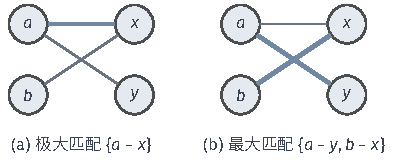
\includegraphics[width=67.07mm]{figures/01-basic-mathematics/04-graphs/tikz/c3-match-maximal-maximum/figure.pdf}
  \caption{极大匹配与最大匹配。细线为允许的配对，粗蓝线为选中的匹配边。(a)$\{a-x\}$已无法再加入任何边，是极大匹配；(b)$\{a-y,b-x\}$的边数更多，是最大匹配。由(a)到(b)须改动已有的配对$a-x$。}
  \label{fig:graph-opt-match-maximal-maximum}
\end{figure}

本节的目标只是最大化$|M|$，边上没有费用；要求完成配对并比较成本的问题留到第~\ref{sec:graph-assignment}节。两侧大小不同时，最大匹配至多有$\min\{|U|,|W|\}$条边，但未必达到这个数：若左侧两个顶点都只与右侧同一个顶点相连，无论怎样选，至多只有一个能配上。下面的构造还依赖两侧的划分。一般的无向图可能含有奇数长的环，例如三角形，它的顶点无法分成两侧使每条边跨侧，下面的单位容量网络构造对它不适用，一般图的匹配需要另外的机制。

\subsection{交替路径与最优性条件}
\label{sec:graph-opt-match-alternating}

图~\ref{fig:graph-opt-match-maximal-maximum}中的改进可以这样描述：从自由顶点$b$出发，先走未选的边$b-x$，再走已选的边$x-a$，最后走未选的边$a-y$到达自由顶点$y$，然后把这条路径上每条边的选中状态取反。下面把这一操作一般化。

给定匹配$M$，若一条路径上的边交替地不属于$M$与属于$M$，称它为\term{交替路径}（alternating path）。两个端点都是自由顶点的交替路径称为关于$M$的增广路径。增广路径的首尾两条边都不在$M$中，因为端点自由；所以路径上不在$M$中的边比在$M$中的边恰好多一条。

\begin{lemma}[沿增广路径翻转]
\label{lem:graph-opt-match-flip}
设$P$是关于匹配$M$的增广路径，把$P$上属于$M$的边移出、不属于$M$的边加入，得到的边集$M'$仍是匹配，且$|M'|=|M|+1$。
\end{lemma}

\begin{proof}
不在$P$上的顶点所关联的选边没有变化。$P$的内部顶点在翻转前恰关联$P$上的一条匹配边和一条非匹配边，翻转后两者互换，仍恰关联一条选边；它不会关联$P$以外的匹配边，因为它在$M$中的唯一配对已经在$P$上。$P$的两个端点原来是自由的，翻转后各关联一条选边。所以$M'$中没有两条边共享端点。由于$P$上非匹配边比匹配边多一条，$|M'|=|M|+1$。
\end{proof}

\paragraph{单位容量网络}
增广路径与第~\ref{sec:graph-max-flow}节的增广路径同名，并非巧合。由二部图构造流网络：增加源点$s$与汇点$t$，从$s$向每个$u\in U$连容量为$1$的弧，每条允许边$u-w$改为容量为$1$的弧$u\to w$，再从每个$w\in W$向$t$连容量为$1$的弧。图~\ref{fig:graph-opt-match-flow-network}画出了一个这样的网络。

给定匹配$M$，在每条匹配边$u-w$对应的路线$s\to u\to w\to t$上各送一单位，得到流值为$|M|$的整数流。反过来，设$\bm x$是一个整数流，每条弧的流量只能是$0$或$1$。顶点$u\in U$只有一条容量为$1$的入弧，流守恒使它至多有一条流量为$1$的出弧；同理，每个$w\in W$至多有一条流量为$1$的入弧。所以流量为$1$的中间弧对应的边两两不共享端点，构成一个匹配，边数等于流值。整数流与匹配就这样一一对应，并且流值等于边数。不能用分数流量四舍五入来代替这一对应：分数流不直接给出配对。

在这个对应下，残量网络中的$s$到$t$简单路径恰好是增广路径。设$\bm x$对应匹配$M$。从$s$出发，正向残量弧$s\to u$存在当且仅当$u$自由；从左侧顶点$u$，可以沿正向残量弧走到任一个与$u$由非匹配边相连的$w$；从右侧顶点$w$，若$w$自由可以走$w\to t$到达汇点，否则只能沿反向残量弧$w\to u'$回到它的配对$u'$，相当于准备撤回匹配边$u'-w$。所以这样一条路径依次经过一个自由左侧顶点、交替的非匹配边与匹配边、一个自由右侧顶点，沿它增广恰好就是引理~\ref{lem:graph-opt-match-flip}中的翻转。

\begin{figure}[!htb]
  \centering
  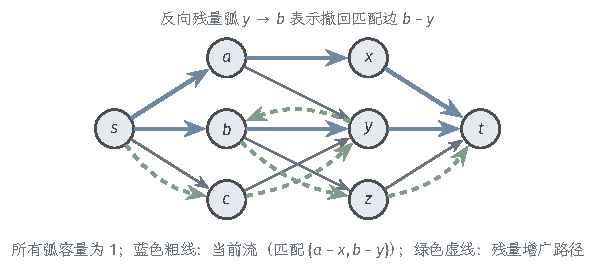
\includegraphics[width=100.76mm]{figures/01-basic-mathematics/04-graphs/tikz/c3-match-flow-network/figure.pdf}
  \caption{二部图匹配的单位容量网络。允许边为$a-x,a-y,b-y,b-z,c-y$，全部弧容量为$1$。蓝色粗弧是匹配$\{a-x,b-y\}$对应的流，流值为$2$。绿色虚线是残量网络中的一条$s$到$t$路径，其中$y\to b$是反向残量弧，表示撤回匹配边$b-y$；这条路径对应交替路径$c-y-b-z$。}
  \label{fig:graph-opt-match-flow-network}
\end{figure}

\paragraph{最大性条件}
有了上面的对应，最大流的判据可以直接搬到匹配上。

\begin{theorem}[增广路径判据]
\label{thm:graph-opt-match-augmenting}
二部图中的匹配$M$是最大匹配，当且仅当不存在关于$M$的增广路径。
\end{theorem}

\begin{proof}
若存在增广路径，由引理~\ref{lem:graph-opt-match-flip}可得更大的匹配，$M$不是最大的。反过来，设不存在增广路径，令$\bm x$是$M$对应的流。由上面的对应，$\bm x$的残量网络中没有$s$到$t$的路径，由第~\ref{sec:graph-max-flow}节的增广路径判据，$\bm x$是最大流。任何匹配$M''$对应一个流值为$|M''|$的流，所以$|M''|\leq\operatorname{val}(\bm x)=|M|$，$M$是最大匹配。
\end{proof}

整数容量时Ford--Fulkerson方法输出整数最大流，所以最大流值总能由某个匹配达到，最大流值就等于最大匹配的边数。

判据与“不能再加一条边”的区别，可以在图~\ref{fig:graph-opt-match-augment}上看清。允许边为$a-x$、$a-y$、$b-y$、$b-z$、$c-y$，当前匹配为$\{a-x,b-y\}$。剩下的三条边$a-y$、$b-z$、$c-y$都与已选边共享端点，所以这个匹配是极大的。但从自由顶点$c$出发，走非匹配边$c-y$、匹配边$y-b$、非匹配边$b-z$，到达自由顶点$z$，得到增广路径$c-y-b-z$。翻转后撤去$b-y$，加入$c-y$与$b-z$，匹配变为$\{a-x,b-z,c-y\}$，大小由$2$增为$3$。

\begin{figure*}[!htb]
  \centering
  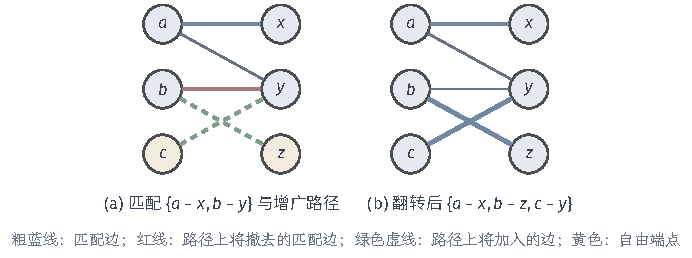
\includegraphics[width=117.094mm]{figures/01-basic-mathematics/04-graphs/tikz/c3-match-augment/figure.pdf}
  \caption{沿交替路径翻转。(a)匹配$\{a-x,b-y\}$是极大匹配，但自由顶点$c$与$z$（黄色）之间有增广路径$c-y-b-z$：绿色虚线为路径上将加入的非匹配边，红线为将撤去的匹配边。(b)翻转后$a-x$保留，$b-y$被$b-z$与$c-y$取代，配对数增加一。}
  \label{fig:graph-opt-match-augment}
\end{figure*}

\subsection{增广匹配算法}
\label{sec:graph-opt-match-algorithm}

定理~\ref{thm:graph-opt-match-augmenting}给出一个算法：只要存在增广路径就沿它翻转，不存在时停止。剩下的问题是怎样在二部图上直接搜索增广路径，而不必显式建立流网络。

算法维护的状态包括：两侧每个顶点的配对伙伴（自由顶点记为空），以及每轮搜索使用的访问标记和右侧顶点的前驱。每轮搜索同时从所有自由左侧顶点出发，用一个队列作广度优先遍历。从左侧顶点$u$出发时，检查它的每个邻居$w$：若$w$尚未访问，则标记$w$并记前驱为$u$；这时若$w$自由，就找到了增广路径，否则把$w$的配对伙伴放入队列，相当于沿匹配边从$w$回到左侧。队列耗尽仍未到达自由右侧顶点，说明当前不存在增广路径。这一搜索恰好就是在单位容量网络的残量网络中从$s$出发的遍历，只是省去了$s$与$t$。

找到自由右侧顶点$w$后，沿前驱回溯：$w$的前驱是左侧顶点$u$，若$u$不自由，再从$u$的原配对伙伴继续回溯，直到到达作为出发点的自由左侧顶点。回溯得到的就是一条增广路径，沿它统一翻转配对伙伴。搜索过程中匹配保持不变，只有完整找到增广路径之后才修改，这样前驱链始终描述同一个匹配下的交替路径。

\begin{algorithm}[增广匹配]
\label{alg:graph-opt-augmenting-matching}
输入：二部图$\mathcal G=(U\cup W,E)$的邻接表。输出：最大匹配$M$，以及最后一次失败搜索的已访问顶点集。状态：两侧顶点的配对伙伴、访问标记、右侧顶点的前驱、队列。
\begin{enumerate}
  \item 令$M=\varnothing$，全部配对伙伴为空。
  \item 清除访问标记，把所有自由左侧顶点放入队列并标记。
  \item 逐个取出左侧顶点$u$，对每个未访问的邻居$w$作标记并令其前驱为$u$；若$w$自由，转第4步，否则把$w$的配对伙伴标记后放入队列。队列耗尽时转第5步。
  \item 从$w$沿前驱与原配对伙伴交替回溯到一个自由左侧顶点，沿这条增广路径翻转配对伙伴，回到第2步。
  \item 输出$M$与本轮的已访问顶点集，停止。
\end{enumerate}
\end{algorithm}

\paragraph{算例}
在图~\ref{fig:graph-opt-match-augment}的二部图上，从$M=\{a-x,b-y\}$开始。自由左侧顶点只有$c$。从$c$检查邻居$y$，记前驱$y\leftarrow c$；$y$已与$b$配对，把$b$放入队列。从$b$检查邻居：$y$已访问，$z$未访问，记前驱$z\leftarrow b$，而$z$自由，找到增广路径。回溯：$z$的前驱是$b$，$b$原来配$y$，$y$的前驱是$c$，$c$自由，路径为$c-y-b-z$。翻转后$c$配$y$，$b$配$z$，$a$仍配$x$，得到大小为$3$的匹配。

下一轮开始时已没有自由左侧顶点，队列一开始就是空的，搜索立即失败，算法停止。这时$|M|=3=|U|$，结论也可以直接从上界看出。若把边$b-z$删去，情形就不同了：从$c$到$y$，再沿匹配边到$b$，$b$的邻居只有已访问的$y$，队列耗尽，不存在增广路径，匹配$\{a-x,b-y\}$就是最大匹配。这里虽然仍有自由顶点$c$与$z$，但不存在连接它们的交替路径，所以不能再改进。对应的残量网络中，从$s$可达的顶点集为$\{s,c,y,b\}$，跨出这一集合的弧是满流的$s\to a$与$y\to t$，割容量为$2$，等于匹配的边数。

\subsection{算法分析与结果检验}
\label{sec:graph-opt-match-analysis}

\paragraph{计算开销}
记$n=|U|+|W|$，$m$为允许边数，$\nu=\min\{|U|,|W|\}$。每次成功的翻转使匹配增加一条边，而匹配至多有$\nu$条边，所以成功的搜索不超过$\nu$次，再加上最后一次失败的搜索。一轮搜索中每个顶点至多入队或标记一次，每条边至多从它的左端点检查一次，所以搜索为$O(n+m)$；回溯与翻转沿一条路径进行，为$O(n)$；初始化配对数组为$O(n)$。总运算量为$O(\nu(n+m))$。还有按层同时寻找多条增广路径的更快的匹配算法，本书不展开，也不引用它们的复杂度界。

\paragraph{结果检验}
检验分两步。可行性：逐条核对所选边都是允许边、任意两条所选边没有公共端点，再重新数出边数。最大性：可以重做一次从全部自由左侧顶点出发的交替搜索，确认到达不了自由右侧顶点；也可以用最后一次失败搜索的已访问顶点集加上$s$构造单位容量网络中的割，核对割容量等于匹配边数，这是一份不依赖算法过程的证书。不能因为每个自由左侧顶点都不与自由右侧顶点直接相连就宣布最大，图~\ref{fig:graph-opt-match-augment}(a)正是这种情形，而那里仍有增广路径。
